\documentclass[11pt]{article}
\usepackage[T1]{fontenc}
\usepackage[utf8]{inputenc}
\usepackage{lmodern}
\usepackage[margin=1in]{geometry}
\usepackage{amsmath,amssymb,amsthm,mathtools}
\usepackage{microtype,booktabs,array,graphicx,xcolor}
\usepackage{enumitem,xurl}
\usepackage[numbers,sort&compress]{natbib}
\usepackage[colorlinks=true,linkcolor=blue!45!black,citecolor=blue!45!black,urlcolor=blue!45!black]{hyperref}
\usepackage[nameinlink,noabbrev]{cleveref}
\hypersetup{pdftitle={Critical-window laws for quadratic relations, code products, and hidden symplectic forms},pdfauthor={Research note prepared for Vladimir Reshetnikov}}
\newcommand{\F}{\mathbb F}
\newcommand{\TV}{\operatorname{TV}}
\newcommand{\qbinom}[2]{\genfrac{[}{]}{0pt}{}{#1}{#2}_q}
\newtheorem{theorem}{Theorem}[section]
\newtheorem{proposition}[theorem]{Proposition}
\newtheorem{lemma}[theorem]{Lemma}
\newtheorem{corollary}[theorem]{Corollary}
\theoremstyle{definition}
\newtheorem{definition}[theorem]{Definition}
\theoremstyle{remark}
\newtheorem{remark}[theorem]{Remark}
\setlist{topsep=4pt,itemsep=3pt}
\setlength{\emergencystretch}{2em}
\allowdisplaybreaks[2]
\title{Critical-window laws for quadratic relations,\\code products, and hidden symplectic forms}
\author{Research note prepared for Vladimir Reshetnikov}
\date{27 November 2026}

\begin{document}
\maketitle
\begin{abstract}
We prove a total-variation universality theorem for the entire solution
space of structured random linear constraints. A uniform Fourier gap,
together with a sufficiently small set of exceptional Fourier directions,
forces the relation space at $D+u$ observations to approach the kernel of
a uniform $(D+u)\times D$ matrix, for every fixed integer $u$.
For arbitrary spaces of homogeneous quadratics in $n$ variables this
applies as soon as $D/(n\log D)\to\infty$, in every characteristic.
Consequently, products of random codes of dimensions $k,\ell$ with
prescribed intersection dimension $i$ have an exact limiting deficiency
law at length $k\ell-\binom i2+u$. This answers a specified asymptotic
regime of Randriambololona's Problem 21 and sharpens the critical case
of the random-square results of Cascudo, Cramer, Mirandola and Z\'emor.
At the exact binary square threshold, the probability of maximal
dimension tends to $0.288788095\ldots$.
We also prove asymptotic independence of the whole corank pattern at
all fixed projective directions in a random space of alternating forms.
Combined with relation-space universality for random two-plane
constraints, this determines the full critical-window experiment for a
hidden symplectic form: the number of compatible nondegenerate forms
has an explicit binomial-mixture law, yielding exact optimal testing and
recovery limits. These results are unconditional. The proof of RH or
Dirichlet GRH is not an assumption of any theorem in this note.
\end{abstract}

\tableofcontents

\section{The advance and its connection to the repository}
\label{sec:intro}

\subsection{What was inspected}
The starting point is the ProveIt directory
\texttt{Analysis/GeneralizedRiemannHypothesis}, pinned at
\begin{center}\small\texttt{b2c37bf49dd792be3258a0925c01725390b2b62f}.\end{center}
Its article index reports 209 consolidated reports and 1,321 theorem-like
statements. The index explicitly describes the consolidation as a merge,
rather than an independent re-verification \cite{ProveItArticle}.
We retrieved the article's section sources and inspected its research
survey, source-mechanism section, and the finite-field spanning and
hidden-form results relevant to this note. We did not independently
check every statement in the collection.

The source-mechanism section separates the upstream RH and Dirichlet-GRH
input from the finite-dimensional ``enough forms'' argument. The latter
motivates a broader question: when many structured random constraints
are imposed, does their solution space behave like the solution space
of fully random equations? The article's hidden-form experiment makes
this question concrete. Its labels
\texttt{spn:thm:hidden-threshold} and
\texttt{spn:thm:hidden-window} establish the sample threshold and a
chi-square limit, while the following text and the open-questions section
leave the full total-variation limit and the distribution of the number
of compatible forms undetermined \cite{ProveItSpanning}.
We answer that question in \cref{thm:complete-critical-law}.

The vendored upstream development is pinned separately at
\begin{center}\small\texttt{72fead102f663d5c7a407964a13dc0cf9d977207}.\end{center}
Its README says that
it is a separate, unbuilt package, and the article's stated input covers
the Riemann zeta function and Dirichlet $L$-functions over $\mathbb Q$.
No upstream Lean build or kernel replay was performed for this note.
That distinction does not affect our proofs: all of them are finite-field
linear algebra, elementary probability, and explicitly justified limits.

\subsection{A result attached to a published problem}
Let $C*C'$ be the span of the coordinatewise products of a vector in
$C$ and a vector in $C'$. Randriambololona asked for the distribution of
its dimension when the intersection dimension of $C,C'$ is prescribed
\cite[Problem~21]{Randriambololona2015}. The correct number of independent
formal products is
\[
 D=k\ell-\binom i2,
 \qquad k=\dim C,\quad\ell=\dim C',\quad i=\dim(C\cap C').
\]
The subtracted term accounts for the duplicate products of distinct
common generators. Put $N=D+u$, the code length, with $u$ fixed.
If $D/((k+\ell-i)\log D)\to\infty$, we prove
\begin{equation}\label{eq:intro-main}
 \Pr\bigl(D-\dim(C*C')=j\mid\dim(C\cap C')=i\bigr)
 \longrightarrow
 \frac{g_\infty q^{-j(j+u)}}{g_jg_{j+u}},
 \quad j\ge\max(0,-u),
\end{equation}
where $g_j=\prod_{r=1}^{j}(1-q^{-r})$ and
$g_\infty=\prod_{r\ge1}(1-q^{-r})$. Convergence holds in total variation
for the entire integer-valued deficiency distribution.

Thus the answer, after the dimensional correction $D$, is universal:
it is independent of the prescribed overlap and of the relative sizes
of the factors within the stated growth range. The square case is
$k=\ell=i$, with $D=k(k+1)/2$. At $N=D$ over $\F_2$, the limiting
probabilities of deficiencies zero, one and two are respectively
\[
 g_\infty=0.288788095\ldots,\qquad
 2g_\infty=0.577576190\ldots,\qquad
 \frac49g_\infty=0.128350264\ldots.
\]
These are asymptotic probabilities; they are not finite-size error
bounds. The earlier random-square theorems already cover diverging
gaps on both sides of this threshold \cite{CCMZ2015}. The new conclusion
determines the bounded-offset transition, including its entire
relation-space distribution.

\subsection{A second exact law, internal to the article's program}
Suppose an unknown nondegenerate alternating form on $\F_q^n$, up to
scale, is observed through independent random two-planes on which it
vanishes. There are $d=\binom n2-1$ projective parameters. In the window
$t=d+a$, with $a$ fixed, let $K$ be the limiting dimension of the
compatible linear space and $Z$ its number of nondegenerate projective
points. Under the unstructured null experiment we prove
\[
 K\sim\pi_{q,a-1},\qquad
 Z\mid K=k\sim\operatorname{Bin}
       \left(\frac{q^k-1}{q-1},\beta_q\right),
 \qquad \beta_q=\prod_{j\ge1}(1-q^{-(2j-1)}).
\]
The likelihood is $Z/\lambda$, with
$\lambda=\beta_q q^{1-a}/(q-1)$. This determines every optimal testing
tradeoff and the optimal probability of recovering the hidden form.
For example, at $q=2,a=0$, the full-observation total variation is
$0.411496025\ldots$, whereas retaining only the solution-space dimension
gives $0.288788095\ldots$. We prove a strict information loss at every
fixed offset and a much larger asymptotic separation below the threshold.

\subsection{Status and prior-art boundaries}
The note gives complete human-readable proofs of the stated theorems.
The uniform-matrix nullity distribution is classical
\cite{Gerth1986,FulmanGoldstein2015}; the assertions to assess for novelty
are its transfer to structured quadratic and plane constraints, the
conditional code-product application, the alternating joint-corank
theorem, and the resulting optimal hidden-form experiment.
The recent unrestricted-matrix MRD argument of the Omega Institute uses
a related tensor-dimension and mixed-moment method \cite{OmegaMRD2026}.
We acknowledge that antecedent explicitly and make no claim to a new
resolution of its MRD-density problem.

The literature comparison in \cref{subsec:code-literature} supports a
proposed new refinement. It does not establish worldwide priority.
Randriambololona's full finite-parameter problem is broader than
\eqref{eq:intro-main}; our result resolves the stated asymptotic regime.
No prominent general conjecture such as nonabelian GRH, Artin's
primitive-root conjecture, or a zero-spacing conjecture is claimed here.
No new theorem in this archive is presented as Lean-formalized.

\section{A criterion for the entire relation space}\label{sec:universality}

Fix a prime power $q$. Write
\[
 g_j=\prod_{i=1}^{j}(1-q^{-i}),\qquad
 g_0=1,\qquad g_\infty=\prod_{i=1}^{\infty}(1-q^{-i})>0.
\]
The Gaussian coefficient $\qbinom{d}{s}$ denotes the number of $s$-dimensional
subspaces of $\F_q^d$ and is zero if $s<0$ or $s>d$. In particular,
\begin{equation}\label{eq:gaussian}
 \qbinom{d}{s}=q^{s(d-s)}\frac{g_d}{g_sg_{d-s}}.
\end{equation}
All limits below keep $q$ and every explicitly fixed integer constant.

Let $E_n$ be an $\F_q$-vector space of dimension $D_n\to\infty$, and let
$\nu_n$ be a probability measure on its dual $E_n^*$. For a fixed nontrivial
additive character $\psi$ of $\F_q$, define
\[
 \widehat\nu_n(A)=\mathbb E_{\ell\sim\nu_n}\psi(\ell(A)),\qquad A\in E_n.
\]
For independent $\ell_1,\ldots,\ell_t\sim\nu_n$, the relation space is
$K_n=\bigcap_{i=1}^{t}\ker\ell_i$. Let $K_n^{\rm unif}$ denote the same
intersection when the functionals are independent and uniform on $E_n^*$.
Total variation here is on the finite set of \emph{all subspaces of the same
space $E_n$}; it retains the position of the subspace, not only its dimension.

\begin{theorem}[Fourier criterion for relation-space universality]\label{thm:abstract}
Suppose that there is a constant $\theta<1$ with
\begin{equation}\label{eq:global-bias}
 \sup_{A\ne0}|\widehat\nu_n(A)|\le\theta+o(1).
\end{equation}
Suppose also that for every $\varepsilon>0$ there are sets
$B_n\subset E_n$, containing zero, such that
\begin{equation}\label{eq:exceptional-bias}
 |B_n|\le q^{\varepsilon D_n+o(D_n)},\qquad
 \sup_{A\notin B_n}|\widehat\nu_n(A)|=o(D_n^{-1}).
\end{equation}
For every fixed $u\in\mathbb Z$, at $t=D_n+u$ one has
\[
 \TV\bigl(\mathcal L(K_n),\mathcal L(K_n^{\rm unif})\bigr)\longrightarrow0.
\]
Moreover, for every fixed $s\ge0$,
\begin{equation}\label{eq:moment-limit}
 \mathbb E\qbinom{\dim K_n}{s}
 \longrightarrow\frac{q^{-s(s+u)}}{g_s}.
\end{equation}
\end{theorem}

\begin{proof}
We give the subspace counting and the inversion argument separately, since
convergence of a few dimension moments alone would not prove the stated conclusion.
Write $D=D_n$. For an $s$-dimensional subspace $S\le E_n$, orthogonality gives
\begin{equation}\label{eq:ps}
 p_n(S):=\Pr(\ell|_S=0)
 =q^{-s}\sum_{A\in S}\widehat\nu_n(A),\qquad
 \Pr(S\le K_n)=p_n(S)^t.
\end{equation}
For each fixed $s$ we first prove the stronger summed estimate
\begin{equation}\label{eq:delta-s}
 \Delta_{n,s}:=\sum_{\dim S=s}\left|p_n(S)^t-q^{-st}\right|\longrightarrow0.
\end{equation}
There is nothing to prove for $s=0$. For $s\ge1$, choose $\varepsilon>0$
so small that, for every $1\le r\le s$,
\begin{equation}\label{eq:epsilon-choice}
 r(1-\varepsilon)>\log_q\bigl(1+(q^r-1)\theta\bigr).
\end{equation}
This is possible because $\theta<1$. Choose $B_n$ as in
\eqref{eq:exceptional-bias}. Classify $S$ by
$r=\dim\langle S\cap B_n\rangle$. If $r=0$, then
\[
 p_n(S)=q^{-s}(1+o(D^{-1})),\qquad
 p_n(S)^t=q^{-st}(1+o(1))
\]
uniformly over these subspaces. Their total contribution to
\eqref{eq:delta-s} tends to zero, since
\begin{equation}\label{eq:baseline-moment}
 \qbinom{D}{s}q^{-st}
 =q^{-s(s+u)}\frac{g_D}{g_sg_{D-s}}
 \longrightarrow\frac{q^{-s(s+u)}}{g_s}.
\end{equation}

If $r\ge1$, select a basis of $\langle S\cap B_n\rangle$ from $B_n$ and
extend it to a basis of $S$. Thus the number of such $S$ is at most
\[
 |B_n|^r q^{(s-r)D}\le q^{(s-r+r\varepsilon)D+o(D)}.
\]
Every element of $S$ outside that $r$-space is outside $B_n$. The triangle
inequality in \eqref{eq:ps} therefore gives
\[
 p_n(S)\le q^{-s}\bigl(1+(q^r-1)\theta+o(1)\bigr).
\]
After raising to $t=D+u$ and summing, the exponent of $q$, apart from $o(D)$,
is
\[
 D\bigl[-r(1-\varepsilon)+
       \log_q(1+(q^r-1)\theta)\bigr],
\]
which is strictly negative by \eqref{eq:epsilon-choice}. The sum of the
comparison terms $q^{-st}$ on these subspaces also tends to zero. This
proves \eqref{eq:delta-s}; summing the inclusion probabilities proves
\eqref{eq:moment-limit}.

We now recover exact subspace probabilities. Put
$\mu_j=(-1)^jq^{j(j-1)/2}$. For a fixed $k$-dimensional subspace $T$ and
integer $L\ge0$, let
\[
 F_{n,L}(T)=\sum_{j=0}^{L}\mu_j
       \sum_{\substack{S\supset T\\\dim S=k+j}}\Pr(S\le K_n).
\]
For $m\ge1$, the finite Gaussian identity
\begin{equation}\label{eq:partial-mobius}
 \sum_{j=0}^{L}\mu_j\qbinom mj
 =(-1)^Lq^{L(L+1)/2}\qbinom{m-1}{L}
\end{equation}
follows by induction from the Gaussian recurrence; it holds with the
zero convention also when $L\ge m$. For $m=0$ the sum is one.
Apply this identity with $m=\dim K_n-k$ on the event $T\le K_n$.
The error $F_{n,L}(T)-\Pr(K_n=T)$ has the same sign $(-1)^L$ for every $T$.
Consequently, after summing absolute errors over all $k$-spaces,
\begin{align}
 &\sum_{\dim T=k}|F_{n,L}(T)-\Pr(K_n=T)|\notag\\
 &\quad\le q^{L(L+1)/2}\qbinom{k+L+1}{k}
       \mathbb E\qbinom{\dim K_n}{k+L+1}.
       \label{eq:mobius-tail}
\end{align}
Indeed, when $m\ge L+1$ one has
$\qbinom{m-1}{L}\le\qbinom m{L+1}$, and
\[
 \qbinom dk\qbinom{d-k}{L+1}
 =\qbinom{k+L+1}{k}\qbinom d{k+L+1}.
\]

For fixed $k,L$, \eqref{eq:delta-s} bounds the difference of the two
truncated inversions, summed over $T$, by
\[
 \sum_{j=0}^{L}|\mu_j|\qbinom{k+j}{k}\Delta_{n,k+j}=o(1).
\]
By \eqref{eq:moment-limit}, the limit of the right side of
\eqref{eq:mobius-tail} is at most
$C_q q^{-L^2/2+O_{k,u}(L)}$, and the identical bound holds for the uniform
model. First let $n\to\infty$ with $L$ fixed, then let $L\to\infty$.
The total absolute difference of exact probabilities over $k$-spaces
therefore tends to zero for every fixed $k$.

Finally, the case $s=1$ of \eqref{eq:moment-limit} gives
$\mathbb E q^{\dim K_n}\to1+q^{-u}$. Thus the dimensions are tight,
uniformly for large $n$, and the same is true in the uniform model.
Truncating the dimension and summing the fixed-$k$ conclusions proves
the total variation assertion.
\end{proof}

\begin{corollary}[Universal bounded-offset nullity law]\label{cor:nullity}
Under the hypotheses of \cref{thm:abstract}, $\dim K_n$ converges in total
variation to the distribution
\begin{equation}\label{eq:pi}
 \pi_{q,u}(k)=
 \frac{g_\infty q^{-k(k+u)}}{g_k g_{k+u}},
 \qquad k\ge\max(0,-u).
\end{equation}
The mass is zero at all other integers. In particular, the probability
that the $t$ constraints have the largest possible rank tends to
\begin{equation}\label{eq:full-rank}
 \frac{g_\infty}{g_{|u|}}=\prod_{j>|u|}(1-q^{-j}).
\end{equation}
\end{corollary}

\begin{proof}
For a uniform $(D+u)\times D$ matrix, counting matrices of rank $D-k$
gives
\[
 \Pr(\dim K_n^{\rm unif}=k)
 =q^{-k(k+u)}\frac{g_Dg_{D+u}}{g_kg_{k+u}g_{D-k}}.
\]
Its limit is \eqref{eq:pi}. Tightness, proved above, shows that these
limits sum to one and gives total variation convergence. Set
$k=\max(0,-u)$ for \eqref{eq:full-rank}.
This last matrix-counting law is classical; the new assertion is its
transfer to the structured constraints below.
\end{proof}

\section{Quadratic evaluations}\label{sec:quadratics}

Let $\mathcal Q_n$ denote the space of homogeneous quadratic polynomials
in $n$ variables over $\F_q$, with basis $X_i^2$ and $X_iX_j$, $i<j$.
Its dimension is $n(n+1)/2$, including in characteristic two. Evaluation
on $\F_q^n$ is injective on this space: evaluation at $e_i$ determines
the square coefficients, and evaluation at $e_i+e_j$ determines each
cross coefficient.

\begin{theorem}[Universality for spaces of quadratics]\label{thm:quadratics}
Let $E_n\le\mathcal Q_n$ be arbitrary subspaces with
$D_n:=\dim E_n\to\infty$ and
\begin{equation}\label{eq:quadratic-size}
 \frac{D_n}{n\log D_n}\longrightarrow\infty.
\end{equation}
For independent uniform points
$x_1,\ldots,x_{D_n+u}\in\F_q^n$, define
\[
 K_n=\{f\in E_n:f(x_j)=0\text{ for every }j\}.
\]
For every fixed integer $u$, the entire subspace $K_n$ has total
variation distance tending to zero from the kernel of a uniform
$(D_n+u)\times D_n$ matrix, under any fixed identification of $E_n$
with $\F_q^{D_n}$. Hence \eqref{eq:pi} and \eqref{eq:full-rank} hold.
The estimates are uniform over the choice of $E_n$ at fixed $n,D_n$.
In particular, any bound $D_n\ge\delta n^2$, with fixed $\delta>0$,
suffices.
\end{theorem}

\begin{proof}
For $f\in\mathcal Q_n$, let
$B_f(x,y)=f(x+y)-f(x)-f(y)$ be its polar bilinear form and put
$r(f)=\operatorname{rank}B_f$. With
$b(f)=\mathbb E_x\psi(f(x))$, differencing gives
\begin{equation}\label{eq:quadratic-bias}
 |b(f)|^2
 =\mathbb E_{h}\psi(f(h))\mathbb E_x\psi(B_f(x,h)),
 \qquad |b(f)|\le q^{-r(f)/2}.
\end{equation}
The inner expectation is one on $\operatorname{rad}B_f$ and zero off it;
on that radical, $\psi\circ f$ is an additive character. This proves the
bound (in fact the squared magnitude is either zero or $q^{-r(f)}$).
In odd characteristic, $r(f)=0$ implies $f=0$. In characteristic two,
$r(f)=0$ means $f=\sum_i a_iX_i^2$; if $f\ne0$, its values are uniform
on $\F_q$ by varying a coordinate with $a_i\ne0$, and $b(f)=0$.
Thus for every nonzero $f$,
\[
 |b(f)|\le q^{-1/2}<1.
\]

We need only a coarse count of low-rank forms. The number of bilinear
forms of rank at most $R$ that are symmetric or alternating is at most
\[
 \qbinom n{n-R}q^{R(R+1)/2}
 \le g_\infty^{-1}q^{nR}.
\]
Here a radical subspace of dimension $n-R$ is selected, and a form on
the quotient is selected; this overcounts and is an upper bound.
In odd characteristic the polar map is injective. In characteristic
two its kernel has dimension $n$. Therefore, in either characteristic,
\begin{equation}\label{eq:lowrank-quadratics}
 \#\{f\in\mathcal Q_n:r(f)\le R\}
 \le g_\infty^{-1}q^{n(R+1)}.
\end{equation}
For a given $\varepsilon>0$, which may be reduced to lie in $(0,1)$,
take $R=\lfloor\varepsilon D_n/(2n)\rfloor$ and
$B_n=\{f\in E_n:r(f)\le R\}$. Equations
\eqref{eq:quadratic-bias}--\eqref{eq:lowrank-quadratics} imply
\[
 |B_n|\le q^{\varepsilon D_n/2+o(D_n)},\qquad
 \sup_{f\notin B_n}|b(f)|\le q^{-(R+1)/2}=o(D_n^{-1}).
\]
Here \eqref{eq:quadratic-size} gives $R/\log D_n\to\infty$ and
$n=o(D_n)$. All estimates are uniform in $E_n$.
Apply \cref{thm:abstract}.
\end{proof}

\section{Constraints from random two-planes}\label{sec:planes}

Let $V=\F_q^n$, with $n$ even, and $E_n=\operatorname{Alt}(V)$, the
$D=\binom n2$-dimensional space of alternating bilinear forms. Alternating
means $A(v,v)=0$ for every $v$, including in characteristic two. A uniform
two-plane can be sampled by a uniform ordered independent pair $(x,y)$;
the equation $A(x,y)=0$ depends only on the plane it spans.

\begin{theorem}[The solution space of random plane constraints]\label{thm:planes}
For $t=D+u$ independent uniform two-planes $L_1,\ldots,L_t\le V$, let
\[
 K_n=\{A\in\operatorname{Alt}(V): A|_{L_j\times L_j}=0
          \text{ for every }j\}.
\]
For every fixed $u\in\mathbb Z$,
\[
 \TV\bigl(\mathcal L(K_n),\mathcal L(K_n^{\rm unif})\bigr)\to0,
\]
where $K_n^{\rm unif}$ is the kernel of independent uniform linear
equations on $\operatorname{Alt}(V)$. Consequently its dimension has
limit \eqref{eq:pi}; conditional on any fixed dimension of positive
limiting probability, its position is asymptotically uniform.
\end{theorem}

\begin{proof}
For $A$ of rank $r$, summing over all ordered pairs first gives
$\sum_{x,y}\psi(A(x,y))=q^{2n-r}$. There are
$(q+1)q^n-q$ linearly dependent ordered pairs, and $A(x,y)=0$ on all of
them. The Fourier coefficient for an independent pair is therefore
\begin{equation}\label{eq:plane-fourier}
 \widehat\nu_n(A)=
 \frac{q^{2n-r}-(q+1)q^n+q}{(q^n-1)(q^n-q)}.
\end{equation}
Every nonzero alternating form has rank at least two, so the global
bound is $q^{-2}+o(1)$. The number with rank at most $R$ is at most
\[
 \qbinom n{n-R}q^{\binom R2}
 \le g_\infty^{-1}q^{nR}.
\]
For $R=\lfloor\eta n\rfloor$ and sufficiently small fixed $\eta>0$,
these form an exceptional set as in \eqref{eq:exceptional-bias}; off
that set \eqref{eq:plane-fourier} is
$O_q(q^{-R}+q^{1-n})=o(D^{-1})$. Apply \cref{thm:abstract}.
\end{proof}

\section{Products of random codes with a prescribed intersection}
\label{sec:code-products}

For vectors $c,c'\in\F_q^N$, write
$c*c'=(c_1c'_1,\ldots,c_Nc'_N)$.  The Schur product of two linear
codes is
\[
 C*C'=\operatorname{span}_{\F_q}\{c*c':c\in C,\ c'\in C'\}.
\]
Its dimension is sensitive to the intersection of the two factors.
The following exact parameterization identifies the relevant quadratic
space and its dimension before any probability estimate is used.

\begin{proposition}[Adapted coordinates for code pairs]
\label{prop:code-parameterization}
Let $0\le i\le\min(k,\ell)$, put $m=k+\ell-i$, and assume $N\ge m$.
There is a space $E_{k,\ell,i}\le\mathcal Q_m$ of dimension
\begin{equation}\label{eq:product-dimension}
 D=k\ell-\binom i2
\end{equation}
with the following property.  Take an $m\times N$ matrix $H$ with
independent uniform entries and condition it to have row rank $m$.
Its rows determine an ordered pair $(C,C')$ uniformly distributed among
all pairs with
\[
 \dim C=k,\qquad \dim C'=\ell,\qquad \dim(C\cap C')=i.
\]
If $h_1,\ldots,h_N\in\F_q^m$ are the columns of $H$, then
\begin{equation}\label{eq:product-evaluation}
 C*C'=\operatorname{im}\bigl(\operatorname{ev}_H:E_{k,\ell,i}
       \longrightarrow\F_q^N\bigr),\qquad
 \operatorname{ev}_H(f)=(f(h_1),\ldots,f(h_N)).
\end{equation}
The probability of the excluded rank-deficiency event is at most
\begin{equation}\label{eq:frame-conditioning}
 \Pr(\operatorname{rank}H<m)
 =1-\prod_{a=0}^{m-1}(1-q^{a-N})
 \le \frac{q^{m-N}}{q-1}.
\end{equation}
\end{proposition}

\begin{proof}
Label the coordinates in $\F_q^m$ by
\[
 z_1,\ldots,z_i,\quad x_1,\ldots,x_{k-i},\quad
 y_1,\ldots,y_{\ell-i}.
\]
Let $E_{k,\ell,i}$ be spanned by all products of one variable from
$(z,x)$ and one from $(z,y)$.  A basis consists of the distinct monomials
\[
 z_a z_b\ (a\le b),\qquad z_a x_b,\qquad z_a y_c,\qquad x_b y_c.
\]
Their number is
\[
 \frac{i(i+1)}2+i(k-i)+i(\ell-i)+(k-i)(\ell-i)
 =k\ell-\frac{i(i-1)}2.
\]
These monomials remain independent as functions over every finite
field, including $\F_2$, by the evaluation observation preceding
\cref{thm:quadratics}.

Use the $z$ and $x$ rows of $H$ to generate $C$, and the $z$ and $y$
rows to generate $C'$.  Full row rank implies that their common
subspace is exactly the span of the $z$ rows.  The coordinatewise
products of these rows are precisely the evaluations of the displayed
monomials, proving \eqref{eq:product-evaluation}.

For a fixed pair $(C,C')$, put $S=C\cap C'$.  A preimage $H$ is specified
by an ordered basis of $S$, an ordered basis of $C/S$ with chosen lifts
in $C$, and an ordered basis of $C'/S$ with chosen lifts in $C'$.
Consequently every pair has exactly
\[
 |\operatorname{GL}_i(q)|\,
 |\operatorname{GL}_{k-i}(q)|\,
 |\operatorname{GL}_{\ell-i}(q)|\,
 q^{i(k+\ell-2i)}
\]
preimages, with $|\operatorname{GL}_0(q)|=1$.  This proves uniformity.
Finally, the usual sequential count of independent rows gives the
product in \eqref{eq:frame-conditioning}; the union bound on its factors
gives the stated upper bound.
\end{proof}

\begin{theorem}[Critical window for products with prescribed overlap]
\label{thm:conditional-products}
Fix a prime power $q$ and an integer $u$.  Let $k,\ell,i$ vary with
$0\le i\le\min(k,\ell)$, and set
\[
 m=k+\ell-i,\qquad D=k\ell-\binom i2,\qquad N=D+u.
\]
Assume $D\to\infty$ and
\begin{equation}\label{eq:product-growth}
 \frac{D}{m\log D}\longrightarrow\infty.
\end{equation}
Choose $C$ and $C'$ independently and uniformly among the
$k$- and $\ell$-dimensional subspaces of $\F_q^N$, and condition on
$\dim(C\cap C')=i$.  Then the relation deficiency
\[
 J=D-\dim(C*C')
\]
converges in total variation to $\pi_{q,u}$ from \eqref{eq:pi}.
In particular, for each fixed $j\ge\max(0,-u)$,
\begin{equation}\label{eq:conditional-product-law}
 \Pr\bigl(\dim(C*C')=D-j\mid\dim(C\cap C')=i\bigr)
 \longrightarrow
 \frac{g_\infty q^{-j(j+u)}}{g_jg_{j+u}},
\end{equation}
and
\begin{equation}\label{eq:conditional-product-maximal}
 \Pr\bigl(\dim(C*C')=\min(N,D)\mid\dim(C\cap C')=i\bigr)
 \longrightarrow \prod_{a>|u|}(1-q^{-a}).
\end{equation}
There is also convergence of the entire relation subspace: in the
random adapted coordinates of \cref{prop:code-parameterization},
$\ker\operatorname{ev}_H\le E_{k,\ell,i}$ has total variation distance
tending to zero from the kernel of an independent uniform $N\times D$
matrix, under the displayed monomial identification of
$E_{k,\ell,i}$ with $\F_q^D$.
\end{theorem}

\begin{proof}
Condition \eqref{eq:product-growth} implies $D/m\to\infty$, so $N\ge m$
eventually and the conditioning in \cref{prop:code-parameterization}
has probability tending to one.  Without that conditioning, the
columns of $H$ are independent uniform points of $\F_q^m$.
Apply \cref{thm:quadratics} to $E_{k,\ell,i}$.  For any random variable
$X$ and event $A$ of positive probability,
\[
 \TV\bigl(\mathcal L(X\mid A),\mathcal L(X)\bigr)\le\Pr(A^c).
\]
Thus \eqref{eq:frame-conditioning} shows that conditioning on full row
rank does not change the asserted limit.  By
\cref{prop:code-parameterization}, this is exactly the prescribed
code-pair distribution.  Taking dimensions is a deterministic map,
which cannot increase total variation.  Now apply \cref{cor:nullity}.
\end{proof}

The position of a relation subspace requires a choice of adapted bases;
the dimension statements do not.  The theorem's last assertion concerns
the explicitly specified random framing, rather than an unspecified
identification attached to an unframed pair of codes.

\begin{corollary}[A simple range, uniform in the intersection]
\label{cor:product-range}
The conclusions of \cref{thm:conditional-products} hold whenever
\begin{equation}\label{eq:simple-product-growth}
 \frac{\min(k,\ell)}{\log(k+\ell)}\longrightarrow\infty,
\end{equation}
uniformly over $0\le i\le\min(k,\ell)$.  In particular they hold when
$k,\ell\to\infty$ and their ratio stays bounded above and bounded
away from zero.
\end{corollary}

\begin{proof}
For every allowed $i$,
\[
 D\ge\tfrac12 k\ell,\qquad m\le k+\ell,\qquad
 \frac{D}{m\log D}
 \ge\frac{\min(k,\ell)}{8\log(k+\ell)}.
\]
Here $k\ell/(k+\ell)\ge\min(k,\ell)/2$ and
$\log D\le2\log(k+\ell)$ were used.  The estimates in
\cref{thm:quadratics} depend on $m,D,q$, not on the particular quadratic
subspace.  The lower bound and the conditioning error therefore tend
to their required limits uniformly in $i$.
\end{proof}

\subsection{Random-generator and full-support versions}

Some formulations of random-code questions sample generator matrices
without initially requiring full row rank.  Even after conditioning on
an atypical intersection, this produces the same asymptotic law here.
This point cannot be justified merely by the unconditional probability
of full rank, because the intersection event itself may be very rare.

\begin{proposition}[Conditioning in the random-generator model]
\label{prop:generator-conditioning}
Let $G\in\F_q^{k\times N}$ and $G'\in\F_q^{\ell\times N}$ be independent
uniform matrices, and let $C,C'$ be their row spaces.  If
$N\ge k+\ell-i$ and $L=N-\max(k,\ell)+i$, then
\begin{align}
 &\Pr\bigl(\dim C<k\text{ or }\dim C'<\ell
       \mid\dim(C\cap C')=i\bigr)\notag\\
 &\qquad\le g_\infty^{-5}
       \left((1-q^{-L-1})^{-2}-1\right).
       \label{eq:conditional-generator-error}
\end{align}
Consequently \cref{thm:conditional-products} also holds for this
random-generator model under its stated growth condition.
\end{proposition}

\begin{proof}
The number of ordered pairs of subspaces with dimensions $r,s$ and
intersection dimension $i$ is
\[
 T_{r,s,i}=\qbinom Nr\qbinom ri\qbinom{N-r}{s-i}
              q^{(r-i)(s-i)}.
\]
For a specified $r$-dimensional row space, the number of $k\times N$
matrices generating it is
$\prod_{a=0}^{r-1}(q^k-q^a)$, which lies between
$g_\infty q^{kr}$ and $q^{kr}$.  From \eqref{eq:gaussian}, each
Gaussian coefficient lies between its leading power of $q$ and
$g_\infty^{-1}$ times that power.  Set $r=k-a$, $s=\ell-b$.
The probability of the rank pair $(r,s)$ together with intersection
dimension $i$, divided by the corresponding probability for $(k,\ell)$,
is therefore at most
\[
 g_\infty^{-5}
 q^{-a(N-k+i+a)-b(N-\ell+i+b)}.
\]
This exponent follows directly by expanding the leading power of
$q$ in $T_{r,s,i}q^{kr+\ell s}$.  Summing over the allowed
$(a,b)\ne(0,0)$ and enlarging the sum to all nonnegative $a,b$ gives
\eqref{eq:conditional-generator-error}, since
$a(N-k+i+a)+b(N-\ell+i+b)\ge(a+b)(L+1)$.
Conditioned further on full row ranks, the pair is the uniform pair
of \cref{thm:conditional-products}.  Under
\eqref{eq:product-growth}, $L\to\infty$, and the error tends to zero.
\end{proof}

One can also require both codes to have full support.  In the
unconditioned adapted-matrix model, the probability that some coordinate
vanishes identically on either code is at most
$N(q^{-k}+q^{-\ell})$.  This tends to zero under
\eqref{eq:product-growth}: indeed $D\le m\min(k,\ell)$, so
$\min(k,\ell)/\log D\to\infty$.  Conditioning on full row rank
changes this bound by a factor tending to one.  Thus requiring full
support leaves the limits in \eqref{eq:conditional-product-law} and
\eqref{eq:conditional-product-maximal} unchanged.

\subsection{Schur squares at the exact threshold}

\begin{corollary}[Square-code critical window]
\label{cor:square-codes}
Fix $q$ and $u\in\mathbb Z$.  Put
$D=k(k+1)/2$, $N=D+u$, and let $k\to\infty$.  If $C$ is uniformly
distributed among the $k$-dimensional codes in $\F_q^N$, then
\[
 D-\dim C^{*2}\ \xrightarrow{\mathrm{TV}}\ \pi_{q,u},
 \qquad C^{*2}=C*C.
\]
The same conclusion holds for the systematic model
$C=\operatorname{rowspan}[I_k\mid A]$, where
$A\in\F_q^{k\times(N-k)}$ has independent uniform entries.
In particular, in either model,
\begin{equation}\label{eq:square-threshold}
 \Pr\bigl(\dim C^{*2}=\min(N,D)\bigr)
 \longrightarrow\prod_{a>|u|}(1-q^{-a});
\end{equation}
at $N=D$, the limiting probability is $g_\infty$, strictly between
zero and one.
\end{corollary}

\begin{proof}
For a uniform code, set $k=\ell=i$ in
\cref{thm:conditional-products}.  Then $C=C'$, $m=k$, and
$D=k(k+1)/2$; the growth condition is automatic.

For the systematic model, the first $k$ evaluation points are
$e_1,\ldots,e_k$.  A quadratic vanishing there has all square
coefficients zero.  Hence the full relation kernel is identified with
the evaluation kernel on
\[
 E_k^0=\operatorname{span}\{X_aX_b:1\le a<b\le k\},\qquad
 D'=\dim E_k^0=\frac{k(k-1)}2,
\]
at the remaining $N-k=D'+u$ independent uniform points.
Theorem~\ref{thm:quadratics} applies to $E_k^0$, and this kernel has
dimension $D-\dim C^{*2}$.  It yields the same law.
\end{proof}

For systematic generators, the entire-kernel comparison takes place
inside $E_k^0$, after the forced diagonal constraints are removed.
An unconstrained uniform kernel in the full $D$-dimensional quadratic
space would be a different comparison model.

\subsection{Published problem and scope of the contribution}
\label{subsec:code-literature}

Randriambololona's Problem~21 asks for estimates of the conditional
distribution of $\dim(C*C')$ given $\dim(C\cap C')=i$
\cite[Section~6, Problem~21]{Randriambololona2015}.
Equations~\eqref{eq:conditional-product-law}--
\eqref{eq:conditional-product-maximal} give its complete limiting
distribution when $N=D+u$, $u$ is fixed, and
\eqref{eq:product-growth} holds.  The proposition on random generators
also covers the matrix model used in that paper.  This is an asymptotic
resolution of a specified regime of the published problem.  The
finite-parameter question for arbitrary $N,k,\ell,i,j$ is not resolved
by these results.  The source's Theorems~16--18
give probability bounds for independent products; they do not state
the conditional bounded-offset law above.

For squares, Cascudo, Cramer, Mirandola and Z\'emor prove that maximal
dimension holds with probability tending to one on either side of the
threshold whenever the gap from $k(k+1)/2$ tends to infinity, however
slowly \cite[Theorems~2.2--2.3]{CCMZ2015}.  At the exact threshold,
their Theorem~2.6 proves that the expected number of quadratic relations,
including zero, tends to $2$; Proposition~5.1 supplies a tail bound.
The fixed-offset law and the systematic-model formulation in
\cref{cor:square-codes} refine this boundary case.  The limiting
distribution itself is the classical uniform-matrix distribution;
its transfer to these dependent quadratic evaluations is the content
of the new argument.

The targeted literature check also examined Chizhov's work on
nonasymptotic filling bounds via generalized Reed--Muller weights
\cite{Chizhov2023}, maximal square dimension for long codes
\cite{Chizhov2025}, and equality of a random subcode's square with the
original code's square in characteristic two \cite{Chizhov2026}.
These works give related probability estimates; the inspected
statements do not give the full bounded-offset distribution or
total-variation convergence of the entire relation space proved here.
This check supports a proposed novelty claim for the stated refinement,
but does not constitute an exhaustive priority review.  No claim is
made here to settle all of Problem~21, higher Schur powers, or a
general conjecture about minimum distances of random product codes.

% Standalone section for incorporation into the main paper.
% All arguments below are independent of Dirichlet GRH.
\section{The whole corank pattern of a random alternating pencil}

Write $\operatorname{Alt}_n(q)$ for the vector space of alternating bilinear
forms on $\mathbb F_q^n$, including zero diagonal in characteristic two. Put
\[
 g_j=\prod_{i=1}^j(1-q^{-i}),\qquad
 g_\infty=\prod_{i\ge1}(1-q^{-i}),\qquad
 \beta_q=\prod_{i\ge1}(1-q^{-(2i-1)}).
\]
All limits in this section keep $q$ and all coefficient directions fixed,
and send $n$ to infinity through even integers.

\begin{theorem}[Joint coranks at every fixed projective direction]
\label{thm:pencil-coranks}
Let $A_1,\ldots,A_k$ be independent uniform elements of
$\operatorname{Alt}_n(q)$. Choose nonzero vectors
$a_1,\ldots,a_s\in\mathbb F_q^k$, no two proportional, and put
$B_i=\sum_j a_{ij}A_j$. Then
\[
 \bigl(\dim\ker B_1,\ldots,\dim\ker B_s\bigr)
 \ \longrightarrow\ (R_1,\ldots,R_s)
\]
in total variation, where the $R_i$ are independent and have distribution
\[
 \Pr(R_i=2h)=\frac{\beta_q q^{-h(2h-1)}}{g_{2h}},
 \qquad h=0,1,2,\ldots.
\]
In particular the nonsingularity indicators are asymptotically independent
Bernoulli variables of parameter $\beta_q$.
\end{theorem}

The independence assertion allows arbitrary linear dependencies among the
coefficient vectors; only distinct projective directions are required.

\begin{lemma}[Strict tensor dimension surplus]
\label{lem:tensor-surplus}
Let $a_i$ be pairwise nonproportional nonzero vectors in a vector space $E$
over any field, and let $W_i$ be finite-dimensional subspaces of another
vector space. Set
\[
 U=\sum_iW_i,\qquad T=\sum_i a_i\otimes W_i\subseteq E\otimes U.
\]
Then $\dim T\ge\dim U$, with equality if and only if the sum of the $W_i$
is direct.
\end{lemma}

\begin{proof}
Pass to an infinite extension field; this preserves dimensions and directness.
Choose $f\in E^*$ nonzero on every $a_i$. Contraction by $f$ maps $T$ onto
$U$, proving the inequality. If the dimensions are equal this contraction
is an isomorphism. Choose $g\in E^*$ so that all ratios
$g(a_i)/f(a_i)$ are distinct; finitely many proper hyperplanes are excluded.
The operator
\[
 (g\otimes1)\circ(f\otimes1)^{-1}:U\longrightarrow U
\]
acts on $W_i$ by the scalar $g(a_i)/f(a_i)$. Eigenspaces with distinct
eigenvalues have direct sum. Conversely a direct sum of the $W_i$ makes the
displayed tensor sum direct, of dimension $\sum_i\dim W_i=\dim U$.
\end{proof}

For $r,m\ge0$ define the number of injective maps
\[
 I_m(r)=\prod_{j=0}^{m-1}(q^r-q^j).
\]
The empty product is one, and $I_m(r)=0$ when $m>r$.

\begin{lemma}[All mixed injection moments]
\label{lem:mixed-injection-moments}
For fixed nonnegative integers $m_1,\ldots,m_s$ and $r_i=\dim\ker B_i$,
\[
 \lim_n\mathbb E\prod_i I_{m_i}(r_i)
   =\prod_i q^{m_i(m_i+1)/2}.
\]
Consequently, for fixed nonnegative integers $\ell_i$,
\[
 \lim_n\mathbb E\prod_i q^{\ell_i r_i}
 =\prod_i M_{\ell_i},\qquad
 M_\ell=\prod_{j=1}^{\ell}(1+q^j).
\]
\end{lemma}

\begin{proof}
Expand the injection counts over tuples of injective maps
$f_i:\mathbb F_q^{m_i}\to\mathbb F_q^n$, and let $W_i$ be their images.
Write $M=\sum_i m_i$.

First suppose the $W_i$ have direct sum. The number of such ordered tuples
of injections is $I_M(n)$. In a basis adapted to their sum, the constraints
$W_i\subseteq\ker B_i$ have total codimension
\[
 M(n-M)+\sum_i\binom{m_i}{2}+2\sum_{i<j}m_im_j
 =nM-\sum_i\frac{m_i(m_i+1)}2.
\]
Indeed, each block joining $W_i$ to the complementary space imposes one
linear condition per entry; each alternating block within $W_i$ imposes
one; and a block joining $W_i$ to $W_j$ imposes two independent conditions,
because $a_i$ and $a_j$ are nonproportional. All underlying upper-triangular
entries of the independent $A_j$ are uniform. The contribution of direct
tuples is therefore
\[
 I_M(n)q^{-nM+\sum_i m_i(m_i+1)/2}
 \longrightarrow q^{\sum_i m_i(m_i+1)/2}.
\]

For a nondirect tuple put $u=\dim\sum_iW_i<M$ and
$v=\dim\sum_i a_i\otimes W_i$. Lemma~\ref{lem:tensor-surplus} gives
$v\ge u+1$. For each of the $n-u$ complementary basis vectors, the
kernel conditions impose $v$ independent linear equations on the
$k\times u$ cross-block entries. These entries for different complementary
vectors are independent. Thus the probability of all kernel conditions
is at most $q^{-v(n-u)}$. The number of tuples spanning a space of dimension
$u$ is at most $C_{q,M}q^{nu}$: choose the $u$-space, then the bounded-size
coordinate matrices of the injections within it. Their contribution is
at most $C_{q,M}q^{-n+v u}$, which tends to zero. There are only finitely many
possible $u,v$ for the fixed moment tuple.

Finally, counting maps by their kernels gives
\[
 q^{\ell r}=\sum_{j=0}^{\ell}\qbinom{\ell}{j} I_j(r).
\]
Apply the first part and the finite $q$-binomial identity
\[
 \sum_{j=0}^{\ell}\qbinom{\ell}{j} q^{j(j+1)/2}
 =\prod_{j=1}^{\ell}(1+q^j).
\]
\end{proof}

\begin{proof}[Proof of Theorem~\ref{thm:pencil-coranks}]
We give the moment-determination step explicitly, since ordinary moment
convergence by itself would not justify this conclusion. Put
\[
 B_q=\prod_{j\ge1}(1-q^{-2j}),\qquad
 C_q^+=\prod_{j\ge1}(1+q^{-j}).
\]
Both are finite positive constants. For fixed $h\ge0$ and $m\ge h$, define
the polynomial in $q^r$
\[
 L_{m,h}(r)=\prod_{\substack{0\le j\le m\\j\ne h}}
            \frac{q^r-q^{2j}}{q^{2h}-q^{2j}}.
\]
Every alternating form in even dimension has even nullity, over every
finite field. On the even values $0,2,\ldots,2m$, this polynomial equals
$\mathbf1_{\{r=2h\}}$. If $r\ge2m+2$ is even, bounding the numerator
factors by $q^r$ and the denominator factors separately above and below
$h$ gives
\[
 |L_{m,h}(r)|
 \le B_q^{-2}q^{mr-m(m+1)-h(h-1)}.
\]
Consequently, at every even $r\ge0$,
\[
 \left|L_{m,h}(r)-\mathbf1_{\{r=2h\}}\right|
 \le E_{m,h}(r):=
 B_q^{-2}q^{-h(h-1)}q^{(m+1)r-(m+1)(m+2)}.
\]
By Lemma~\ref{lem:mixed-injection-moments}, all fixed mixed moments of
these error majorants factor in the limit. Moreover,
\[
 \lim_n\mathbb E E_{m,h}(r_i)
 \le B_q^{-2}C_q^+q^{-h(h-1)}q^{-(m+1)(m+2)/2}
 =:\varepsilon_{m,h}\longrightarrow0,
\]
since $M_{m+1}\le C_q^+q^{(m+1)(m+2)/2}$.
For fixed $h_1,\ldots,h_s$, the difference between the product of the
indicators and the product of the polynomials is bounded by
$\prod_i(1+E_{m,h_i}(r_i))-1$. Its limiting expected value is at most
$\prod_i(1+\varepsilon_{m,h_i})-1$, tending to zero with $m$.
The mixed polynomial expectations factor in the limit, again by the
mixed moment lemma. Thus each joint point probability converges to the
product of its marginal limits.

For completeness, choosing the radical and then a nondegenerate form on
the quotient gives, for even $r\le n$,
\[
 \Pr(\dim\ker A_1=r)
 =\qbinom{n}{r}
 q^{\binom{n-r}{2}-\binom n2}
 \prod_{j=1}^{(n-r)/2}(1-q^{-(2j-1)}).
\]
Its limit is $\beta_q q^{-r(r-1)/2}/g_r$. The first moment bound
$\mathbb E q^{r_i}\to q+1$ makes the marginals tight, so these probabilities
sum to one. Joint tightness follows by a union bound. Pointwise
convergence on the countable state space, together with tightness, gives
total-variation convergence.
\end{proof}

\begin{corollary}[A random finite-dimensional space of alternating forms]
\label{cor:binomial-pencil}
Let $U_n$ be a uniformly chosen $k$-dimensional subspace of
$\operatorname{Alt}_n(q)$, where $k$ is fixed. Put
$m_k=(q^k-1)/(q-1)$, and let $Z(U_n)$ be the number of its projective points
represented by nonsingular forms. Then
\[
 Z(U_n)\longrightarrow\operatorname{Bin}(m_k,\beta_q)
\]
in total variation. More strongly, with respect to a uniformly chosen
ordered basis of $U_n$, the entire projective corank pattern converges to
independent copies of the distribution in Theorem~\ref{thm:pencil-coranks}.
In particular,
\[
 \Pr(\text{every nonzero form of }U_n\text{ is nonsingular})
 \longrightarrow\beta_q^{m_k}.
\]
\end{corollary}

\begin{proof}
Independent uniform $A_1,\ldots,A_k$ are linearly independent with
probability $\prod_{j=0}^{k-1}(1-q^{j-\binom n2})\to1$. Conditioning on
that event gives a uniform ordered basis of a uniform $k$-space. Apply
the theorem to one representative of every point of
$\mathbb P^{k-1}(\mathbb F_q)$. The case $k=0$ is interpreted with zero
projective points.
\end{proof}

\paragraph{Relation to prior work.}
The tensor-dimension mechanism has a closely related unrestricted-matrix
antecedent in the November 2026 Omega Institute proof of the fixed-field
column limit for MRD-code densities \cite{OmegaMRD2026}. That work uses mixed kernel moments
and finite Mobius inversion to establish joint zero-nullity probabilities.
Here the matrices are alternating, every nullity has fixed parity, and
the conclusion determines the entire projective corank pattern. The
explicit interpolation argument above is included to establish this
stronger distributional statement without importing a moment-uniqueness
theorem. This comparison is a targeted prior-art check, not a claim of
exhaustive priority verification.

\section{The exact hidden-form experiment in its critical window}

Fix a prime power $q$, let $n\ge4$ tend to infinity through even integers, and
put $D=\binom n2$ and $d=D-1$. Let $\mathcal H_n$ be the projective
nondegenerate alternating forms on $\mathbb F_q^n$, and let
$\mathcal G_n=\operatorname{Gr}(2,\mathbb F_q^n)$. Under the null law
$Q_{n,t}$ the observed planes are independent and uniform on $\mathcal G_n$.
Under the planted law $P_{n,t}$ a uniform $[H]\in\mathcal H_n$ is chosen
once, and the planes are conditionally independent uniform $H$-isotropic
planes. Define the compatible linear space
\[
 \mathcal N=\{G\in\operatorname{Alt}_n(q):G|_{K_i\times K_i}=0
                 \text{ for all observed }K_i\},
\]
and let $Z_n$ be the number of projective nondegenerate forms in
$\mathcal N$. We use
\[
 c_q=\prod_{j\ge2}(1-q^{-(2j-1)})=\frac{\beta_q}{1-q^{-1}},
 \qquad g_j=\prod_{i=1}^j(1-q^{-i}),\qquad g_0=1.
\]

For each integer $b$, define a probability distribution on
$k\ge\max(0,-b)$ by
\[
 \pi_{q,b}(k)=\frac{g_\infty q^{-k(k+b)}}{g_kg_{k+b}}.
\]
This is the limiting nullity law of \cref{cor:nullity}, with $b=u$. Write
$m_k=(q^k-1)/(q-1)$.

\begin{theorem}[Complete critical law and optimal inference]
\label{thm:complete-critical-law}
Fix an integer $a$, put $t=d+a$ and $\lambda=c_qq^{-a}$, and define a
limiting pair $(K,Z)$ by
\[
 \Pr(K=k)=\pi_{q,a-1}(k),\qquad
 (Z\mid K=k)\sim\operatorname{Bin}(m_k,\beta_q).
\]
Then under $Q_{n,d+a}$,
\[
 (\dim\mathcal N,Z_n)\longrightarrow(K,Z)
\]
in total variation. Under the planted law, the limiting pair instead has
\[
 \Pr(K=k)=\pi_{q,a}(k-1),\qquad
 (Z\mid K=k)\sim1+\operatorname{Bin}(m_k-1,\beta_q),
 \qquad k\ge1.
\]
The exact limiting full-observation total variation is
\begin{align*}
 T_q(a)
 &=\lim_n\operatorname{TV}(P_{n,d+a},Q_{n,d+a})\\
 &=\mathbb E(1-Z/\lambda)_+
  =\frac12\mathbb E|Z/\lambda-1|\\
 &=\sum_{k\ge\max(0,1-a)}\pi_{q,a-1}(k)
   \sum_{z=0}^{m_k}\binom{m_k}{z}\beta_q^z(1-\beta_q)^{m_k-z}
                         (1-z/\lambda)_+.
\end{align*}
For $a\ge0$ this reduces to the positive series
\[
 T_q(a)=\sum_k\pi_{q,a-1}(k)(1-\beta_q)^{m_k}.
\]
The limiting optimal probability of recovering the hidden projective form is
\[
 S_q(a)=\frac{1-\sum_k\pi_{q,a-1}(k)(1-\beta_q)^{m_k}}{\lambda}.
\]
The limiting probability that there is a unique compatible nondegenerate
projective form is
\[
 U_q(a)=\frac{\beta_q}{\lambda}
     \sum_{k\ge1}\pi_{q,a-1}(k)m_k(1-\beta_q)^{m_k-1}.
\]
At each finite size the optimal equal-prior test compares $Z_n$ to
$\lambda_n=|\mathcal H_n|p_n^t$, where
\[
 p_n=\frac{q^{n-2}-1}{q^{n-1}-1}.
\]
Thus counting the compatible nondegenerate forms retains all information
for testing. For $a\ge0$, accepting the planted model exactly when
$Z_n>0$ is already optimal at every $n\ge4$.
\end{theorem}

\begin{proof}
The exact group-orbit and plane counts give
\[
 |\mathcal H_n|=q^{D-1}c_n,\qquad
 c_n=\prod_{j=2}^{n/2}(1-q^{-(2j-1)}),\qquad
 \frac{dP_{n,t}}{dQ_{n,t}}=\frac{Z_n}{\lambda_n}.
\]
The first identity follows by dividing the number of nondegenerate
alternating forms by $q-1$. For a fixed $H$, count ordered independent
vectors $(u,v)$ with $H(u,v)=0$ to obtain $p_n$; this probability does not
depend on $H$. Each compatible projective form contributes the same
conditional density $p_n^{-t}$, proving the likelihood formula.
Since $p_n=q^{-1}(1+O_q(q^{2-n}))$ and $t=O(n^2)$,
$\lambda_n\to c_qq^{-a}=\lambda$.

Theorem~\ref{thm:planes} makes the law of $\mathcal N$ under $Q$
asymptotically the law of the kernel of a uniform $t\times D$ matrix.
Conditional on its dimension, that latter kernel is uniform among
subspaces of that dimension. Its dimension tends to $\pi_{q,a-1}$.
Corollary~\ref{cor:binomial-pencil} gives the conditional binomial limit
for each fixed dimension. Truncating the tight dimension distribution
proves total-variation convergence of the pair.

For this null limit,
\[
 \mathbb E q^K=1+q^{1-a},\qquad
 \mathbb E m_K=\frac{q^{1-a}}{q-1},\qquad
 \mathbb EZ=\beta_q\mathbb E m_K=c_qq^{-a}=\lambda.
\]
The first identity follows either by summing $\pi_{q,a-1}$ or by counting
nonzero kernel vectors in the uniform rectangular matrix model.
The planted limit has point masses $z/\lambda$ times the null point
masses. They sum to one by the last identity. Pointwise convergence of
the exact likelihood-weighted masses, followed by preservation of total
mass, gives total-variation convergence under the planted law too.
Size-biasing a binomial variable gives $1+\operatorname{Bin}(m_k-1,\beta_q)$.
The size-biased dimension weight is
\[
 \pi_{q,a-1}(k)\frac{\beta_qm_k}{\lambda}
 =\pi_{q,a-1}(k)q^{a-1}(q^k-1)=\pi_{q,a}(k-1).
\]

For any likelihood $L$, total variation equals
$\mathbb E_Q(1-L)_+$. This is a bounded continuous function of $L$, so
the convergence just proved yields $T_q(a)$ directly. Since
$\mathbb EZ=\lambda$, the absolute-value form follows as well. If $a\ge0$
then $0<\lambda<1$, so only $Z=0$ contributes. At finite size one has
$p_n<q^{-1}$ and $c_n<1$ for $n\ge4$, whence
$\lambda_n<c_nq^{-a}<1$ and the same testing rule is exactly optimal.

The posterior distribution of $[H]$ is uniform over the $Z_n$ compatible
nondegenerate forms. Hence the optimal recovery success is
\[
 \mathbb E_P(1/Z_n)
 =Q_{n,t}(Z_n>0)/\lambda_n.
\]
This proves the recovery formula. Similarly,
$P_{n,t}(Z_n=1)=Q_{n,t}(Z_n=1)/\lambda_n$, giving the uniqueness formula.
\end{proof}

\paragraph{Arbitrary prior probabilities.}
If the prior probability of the planted law is $\theta\in(0,1)$, its
optimal limiting Bayes error is
\[
 \mathbb E\min\{1-\theta,\theta Z/\lambda\}.
\]
At finite size the optimal test accepts the planted model when
$Z_n/\lambda_n>(1-\theta)/\theta$, with either decision allowed at a tie.
This follows from the same exact likelihood and requires no further
limit theorem.

\paragraph{A rigorous truncation bound.}
For $r\ge\max(1,1-a)$,
\[
 \Pr(K\ge r)\le\mathbb E\qbinom{K}{r}
 =\frac{q^{r(1-a)-r^2}}{g_r}.
\]
The identity follows from counting the $r$-spaces in a uniform matrix
kernel before taking its dimension to infinity. Thus truncating the
positive series for $T_q(a)$ before $k=r$ incurs error no larger than the
displayed bound; the same statement holds for the bounded-summand formula
when $a<0$. Product tails may be enclosed by
$1-\sum_{j>J}q^{-j}\le\prod_{j>J}(1-q^{-j})\le1$, with the analogous
odd-index bound for $\beta_q$.

\begin{corollary}[Exact distinction from dimension-only inference]
\label{cor:dimension-gap}
The limiting total variation when only $\dim\mathcal N$ is retained is
\[
 T_q^{\rm dim}(a)=
 \begin{cases}
 q^{a-1}g_\infty/g_{1-a},&a\le0,\\
 g_\infty/g_{a-1},&a\ge1.
 \end{cases}
\]
For every fixed integer $a$, the full-observation distance is strictly
larger than the dimension-only distance. As $a\to-\infty$ after the
critical-window limit,
\[
 T_q(a)\sim\sqrt{\frac{1-\beta_q}{2\pi c_q}}\,q^{a/2},
 \qquad T_q^{\rm dim}(a)\sim q^{a-1}.
\]
\end{corollary}

\begin{proof}
The dimension likelihood is
$\mathbb E(Z/\lambda\mid K=k)=q^{a-1}(q^k-1)$.
For $a\le0$ put $h=1-a\ge1$. The smallest possible null dimension is $h$;
its likelihood is $1-q^{-h}<1$, whereas all larger dimensions have
likelihood greater than one. Thus the distance is
$q^{-h}\pi_{q,-h}(h)=q^{a-1}g_\infty/g_{1-a}$.
For $a\ge1$, only $k=0$ has likelihood below one, except the harmless tie
at $q=2,a=1,k=1$. This gives $\pi_{q,a-1}(0)=g_\infty/g_{a-1}$.

For strictness, choose any sufficiently large $k$ with positive
$\pi_{q,a-1}(k)$ and $m_k>\lambda$. Conditional on that dimension, the
binomial variable has positive probability both at $0$ and above
$\lambda$. The function $(1-x/\lambda)_+$ is therefore strictly above
its Jensen value after averaging over that conditional distribution.
Summing gives a strict gap.

For the asymptotic formula put $h=1-a\to\infty$. Then
\[
 \Pr(K=h)=g_\infty/g_h=1-O_q(q^{-h}),\qquad
 \lambda=\frac{\beta_qq^h}{q-1}.
\]
On $K=h$, $Z$ is binomial with $m_h=(q^h-1)/(q-1)$ trials, mean
$\lambda-\beta_q/(q-1)$ and variance asymptotic to
$(1-\beta_q)\lambda$. The usual binomial central limit theorem, together
with bounded second moments of its normalized version, gives
\[
 \mathbb E|Z-\lambda|\sim
 \sqrt{2/\pi}\sqrt{(1-\beta_q)\lambda}
\]
for this conditional binomial law. The omitted dimensions contribute
only $O_q(\lambda^{-1})$ to the normalized absolute-value expectation:
indeed
\[
 \mathbb E[m_K;K>h]
 =\frac{q^h}{q-1}-\frac{q^h-1}{q-1}\frac{g_\infty}{g_h}=O_q(1),
\]
and $\Pr(K>h)=O_q(q^{-h})=O_q(\lambda^{-1})$.
Dividing by $2\lambda$ proves the first asymptotic; the exact dimension
formula gives the second.
\end{proof}

\paragraph{Optimal inference with bounded expected enumeration.}
Compute a basis of $\mathcal N$ by Gaussian elimination, enumerate its
projective points, and test the corresponding alternating matrices for
nonsingularity. This computes $Z_n$ and hence the optimal test and the
uniform posterior exactly. At every fixed critical offset, the expected
number of enumerated points stays bounded under both hypotheses.
Under $Q$ this follows from the first subspace moment; under $P$, the
likelihood identity bounds it by a constant times the first two subspace
moments under $Q$, using $m_K^2=m_K+q(q+1)\qbinom K2$.
The nullspace computation costs $O(n^6)$ field
operations and each determinant test costs $O(n^3)$, so the complete
optimal procedure has expected $O_{q,a}(n^6)$ field-operation cost.
The limiting success probability of elimination alone is $g_\infty/g_a$
for $a\ge0$ and zero for $a<0$, since its success event under the planted
law is $\dim\mathcal N=1$. This expectation statement concerns the
specified random experiments; the worst-case nullspace can be large.

\paragraph{Numerical example.}
For $q=2$, at the parameter-count threshold $t=D-1$ ($a=0$),
\[
 \begin{array}{ll}
 T_2(0)=0.411496025790588369\ldots,&
 T_2^{\rm dim}(0)=0.288788095086602421\ldots,\\
 S_2(0)=0.701564718009178670\ldots,&
 U_2(0)=0.488389858128608926\ldots.
 \end{array}
\]
Elimination alone recovers a unique linear form with limiting probability
$\prod_{j\ge1}(1-2^{-j})=0.288788095086602421\ldots$. Checking nondegeneracy resolves
additional cases, and even when several compatible nondegenerate forms
remain, choosing one uniformly achieves the optimal success $S_2(0)$.

\section{Verification, numerical evaluation, and reproducibility}
\label{sec:verification}

The asymptotic theorems are proved in the preceding sections. The
accompanying computations have three separate purposes: exact checks of
finite identities, certified evaluation of the proved limiting formulas,
and illustrations of finite-size convergence. None substitutes for the
proof of an asymptotic statement.

\subsection{Exact finite-field checks}
The standard-library Python program \texttt{code/verify\_exact.py} uses
integer and rational arithmetic, with an explicit implementation of
$\F_4=\F_2[z]/(z^2+z+1)$. Its recorded run passed the following checks.
\begin{center}
\begin{tabular}{@{}lr@{}}
\toprule
Identity or finite assertion & Cases\\
\midrule
Quadratic Fourier identities and polar radicals & 163\\
Plane Fourier identities on all alternating four-dimensional forms & 4,889\\
Partial Gaussian M\"obius identity & 495\\
Flag-count identity & 1,365\\
Uniform-matrix subspace moments & 2,178\\
Uniform-matrix rank-law normalization & 363\\
\bottomrule
\end{tabular}
\end{center}
The alternating-form tests exhaust all forms in dimension four over
$\F_2,\F_3,\F_4$; the quadratic tests exhaust the stated small spaces,
including nonzero pure-square forms in characteristic two. The program
also checks the truncation inequality and the nondegenerate-form count.
The exact list of parameters and scope is in
\texttt{results/exact\_checks.json}.

\subsection{Certified limiting profiles}
The program \texttt{code/compute\_profiles.py} evaluates the limiting
formulas for $q=2,3,4,5$ and $-5\le a\le5$.
Its 44 computations use 100-digit outward-rounded interval arithmetic,
400 factors for each infinite product, and the explicit Gaussian-moment
tail bound from the hidden-form section. Each saved decimal is enclosed
with absolute error at most $10^{-45}$. The dimension-tail bound in
each run is below $10^{-70}$. These are error bounds for the infinite
\emph{limit formulas}, not rates of convergence from finite $n$.

\begin{table}[htbp]
\centering\small
\begin{tabular}{@{}rrrrrr@{}}
\toprule
$q$ & $a$ & Full TV & Dimension TV & Recovery & Elimination \\
\midrule
2 & -3 & 0.14010654 & 0.05867441 & 0.14897429 & 0.00000000 \\
2 & -2 & 0.20466458 & 0.11001451 & 0.29218681 & 0.00000000 \\
2 & -1 & 0.29754118 & 0.19252540 & 0.50331096 & 0.00000000 \\
2 & 0 & 0.41149603 & 0.28878810 & 0.70156472 & 0.28878810 \\
2 & 1 & 0.64934993 & 0.28878810 & 0.83603079 & 0.57757619 \\
2 & 2 & 0.80832002 & 0.57757619 & 0.91401872 & 0.77010159 \\
2 & 3 & 0.89976122 & 0.77010159 & 0.95596960 & 0.88011610 \\
3 & 0 & 0.30597981 & 0.28006304 & 0.72406387 & 0.56012608 \\
4 & 0 & 0.24107857 & 0.22951251 & 0.77177168 & 0.68853754 \\
5 & 0 & 0.19642113 & 0.19008320 & 0.81032945 & 0.76033280 \\
\bottomrule
\end{tabular}
\caption{Selected limiting probabilities. Recovery is the optimal posterior success probability; elimination requires a one-dimensional compatible linear space. The full 44-profile table is included as CSV and JSON. Displayed digits are rounded from certified evaluations.}
\label{tab:selected-profiles}
\end{table}


\begin{figure}[htbp]
 \centering
 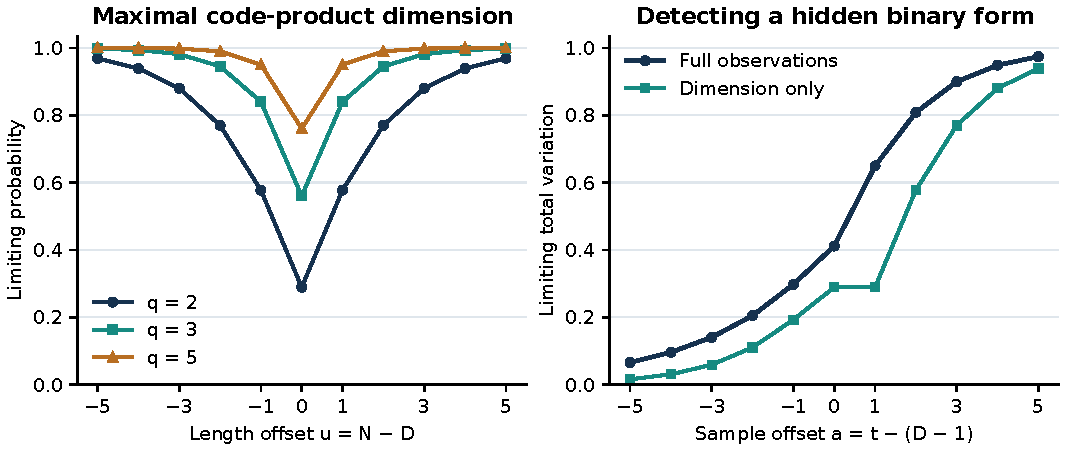
\includegraphics[width=\linewidth]{results/critical_profiles.pdf}
 \caption{Left: the limiting probability that a code product attains
 its maximal possible dimension at offset $u$ from its corrected
 dimension $D$. Right: the hidden binary-form testing limit, comparing
 full observations with the dimension statistic alone. Each plot shows
 proved formulas; the curves join discrete integer offsets.}
 \label{fig:profiles}
\end{figure}

\subsection{Finite-size illustrations}
The standard-library program \texttt{code/simulate\_binary.py} samples
actual binary square codes and actual random-plane constraints. Its
recorded run uses seed 20261127 and 1,500 trials per parameter setting,
27,000 samples in total. The output includes frequencies, Monte Carlo
standard errors, and the exact finite-size likelihood normalization for
the hidden-form experiment. Small dimensions can be far from the limit:
zero or repeated generator columns are among the finite-size effects
that disappear asymptotically. No finite-size accuracy guarantee is
inferred from these simulations.

\subsection{Proof dependency and formalization notes}
The logical route starts with Fourier separation, which gives summed
estimates for subspace inclusions. M\"obius inversion with a controlled
tail then gives universality for the entire kernel.
Quadratic character sums and low-rank counts supply the two hypotheses
for evaluations; the exact plane Fourier identity supplies them for
alternating constraints. The code applications then use an exact
adapted-basis count. For the hidden-form law, the additional ingredient
is the joint-corank theorem, whose independent ingredients are tensor
dimension surplus, mixed injection moments, and interpolation on even
nullities. The final statistical conclusions follow from an exact
likelihood and binomial size biasing.

The archive includes \texttt{FORMALIZATION\_NOTES.txt}, which identifies
these modules and their theorem statements for a future Lean development.
It is a roadmap, not an executable or checked Lean proof. The finite
checkers are executable verification of the identities they enumerate.
The LaTeX source is the complete human-readable proof.

\subsection{Rebuilding}
From the archive root, the commands are
\begin{verbatim}
python3 code/verify_exact.py
python3 code/compute_profiles.py
python3 code/simulate_binary.py --trials 1500
python3 code/make_figure.py
latexmk -pdf -interaction=nonstopmode -halt-on-error critical_window_laws.tex
\end{verbatim}
The exact checker and simulator need only Python's standard library.
The profile computation needs \texttt{mpmath}; the optional plotting
step needs \texttt{matplotlib}. The recorded outputs and figure are
already included, so the PDF can be rebuilt without rerunning numerical
computations. Standard LaTeX packages, BibTeX, and \texttt{latexmk}
suffice for the document build.


\bibliographystyle{plainnat}
{\raggedright\bibliography{references,code_product_refs}}
\end{document}
